\hypertarget{kalman-filter-for-2-wheeled-mobile-robots}{%
\section{Kalman Filter for 2-wheeled mobile
robots}\label{kalman-filter-for-2-wheeled-mobile-robots}}

\hypertarget{robotic-systems-course-project---20222023}{%
\subsubsection{Robotic systems course project -
2022/2023}\label{robotic-systems-course-project---20222023}}

\hypertarget{introduction}{%
\subsection{Introduction}\label{introduction}}

Kalman filter is a predictive filter based on a model of the behaviour
of the system. The aim of predictive filter is to reduce the measurement
error on the basis of the knowledge of the system model.

In order to accomplish that goal, the filter firstly performs an
estimate of the state variable of the system and compares it with sensor
data. The resulting error is then cyclically reduced through a PI
controller in which the proportional constant (\emph{Kp}) is updated at
each iteration.

Eventually, the output of the controller is used to correct the
prediction and the filter restarts.

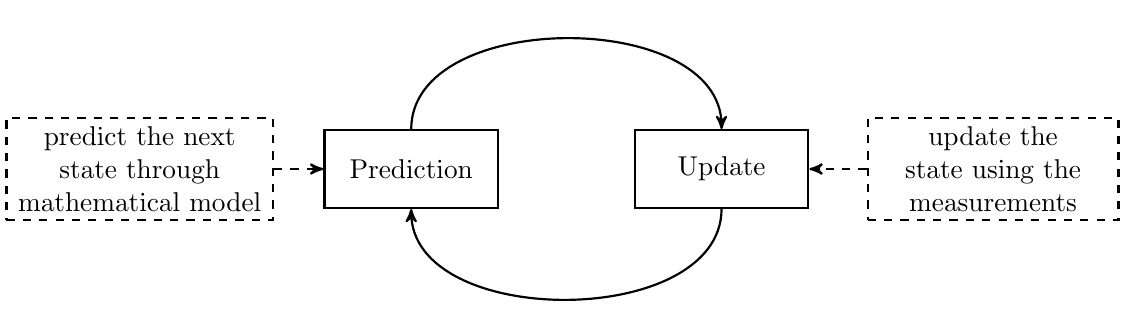
\includegraphics{pics/kf.png}

Our project consists in designing a Kalman filter for our two-wheeled
robots, in order to make values from the optical encoders more
trustworthy.

\hypertarget{software}{%
\subsection{Software}\label{software}}

The Kalman Filter need some matrices in order to work:

\begin{itemize}
\tightlist
\item
  X is the state vector; it contains the state variables of the model:
\end{itemize}

\[
X = \begin{bmatrix}
x_R \\
y_R \\
\theta_R
\end{bmatrix}
\]

\begin{itemize}
\tightlist
\item
  Q is the covariance matrix of the uncertainty of the system; in its
  main diagonal, there are the variance values of the state variable:
\end{itemize}

\[
Q = \begin{bmatrix}
\sigma_{x_R}^2 & 0 & 0 \\
0 & \sigma_{y_R}^2 & 0 \\
0 & 0 & \sigma_{\theta_R}^2
\end{bmatrix}
\]

\begin{itemize}
\tightlist
\item
  R is the covariance matrix of the uncertainty of the measure; in its
  main diagonal, there are the variance values of the state variable:
\end{itemize}

\[
R = \begin{bmatrix}
\sigma_{x_E}^2 & 0 & 0 \\
0 & \sigma_{y_E}^2 & 0 \\
0 & 0 & \sigma_{\theta_E}^2
\end{bmatrix}
\]

\begin{itemize}
\tightlist
\item
  H is the matrix that specifies the state variables measured (in this
  case the y component):
\end{itemize}

\[
H = \begin{bmatrix}
0 & 0 & 0 \\
0 & 1 & 0 \\
0 & 0 & 0
\end{bmatrix}
\]

\begin{itemize}
\tightlist
\item
  P is the covariance error matrix;
\item
  K is the optimal gain (the proportional constant).
\end{itemize}

\begin{center}\rule{0.5\linewidth}{0.5pt}\end{center}

The complete algorithm is shown as follows:

\begin{itemize}
\tightlist
\item
  \textbf{\emph{Prediction}}
\end{itemize}

During the prediction step, we initialized the the state matrix A and
the state vector x̂ using the mathematical models of a two-wheeled robot.
\[
x̂ = A x̂
\]

\begin{itemize}
\tightlist
\item
  \textbf{\emph{Update of error covariance}}
\end{itemize}

The error covariance matrix P is determined from the covariance matrix
Q. \[
P = A P A^T + Q
\]

\begin{itemize}
\tightlist
\item
  \textbf{\emph{Optimal gain}}
\end{itemize}

Then K is computed such that P is minimal. \[
K = P H^T (H P H^T + R)^{-1}
\]

\begin{itemize}
\tightlist
\item
  \textbf{\emph{Measure correction}}
\end{itemize}

Starting from the updated K and the prediction given by the model, we
correct the measure from the sensor. \[
x̂ = x̂ + K (z − H x̂)
\]

\begin{itemize}
\tightlist
\item
  \textbf{\emph{Error covariance correction}}
\end{itemize}

\[
P = (I − K H) P
\]

The algorithm is iteratively repeated for all the duration of the
sampling.

\begin{center}\rule{0.5\linewidth}{0.5pt}\end{center}

\hypertarget{matrix.cpp}{%
\subsubsection{Matrix.cpp}\label{matrix.cpp}}

Since there is no numpy in C++, we decided to implement our own library
for handling the matrix operations involved within the Kalman algorithm.

\hypertarget{constructor}{%
\paragraph{Constructor}\label{constructor}}

It is possible to make matrices and vectors of any dimension by just
indicating the number of rows, the number of columns and the elements
within an array.

\begin{Shaded}
\begin{Highlighting}[]
\NormalTok{Matrix }\OperatorTok{(}\DataTypeTok{unsigned} \DataTypeTok{int}\NormalTok{ \_num\_rows}\OperatorTok{,} \DataTypeTok{unsigned} \DataTypeTok{int}\NormalTok{ \_num\_cols}\OperatorTok{,} \DataTypeTok{double}\NormalTok{ \_matrix}\OperatorTok{[])}
            \OperatorTok{:}\NormalTok{ num\_cols}\OperatorTok{\{}\NormalTok{\_num\_cols}\OperatorTok{\},}\NormalTok{ num\_rows}\OperatorTok{\{}\NormalTok{\_num\_rows}\OperatorTok{\}}
        \OperatorTok{\{}
\NormalTok{            matrix }\OperatorTok{=} \KeywordTok{new} \DataTypeTok{double}\OperatorTok{*[}\NormalTok{num\_rows}\OperatorTok{];}
            \ControlFlowTok{for}\OperatorTok{(}\DataTypeTok{unsigned} \DataTypeTok{short}\NormalTok{ i}\OperatorTok{=}\DecValTok{0}\OperatorTok{;}\NormalTok{ i}\OperatorTok{\textless{}}\NormalTok{num\_rows}\OperatorTok{;}\NormalTok{ i}\OperatorTok{++)\{}
\NormalTok{                matrix}\OperatorTok{[}\NormalTok{i}\OperatorTok{]} \OperatorTok{=} \KeywordTok{new} \DataTypeTok{double}\OperatorTok{[}\NormalTok{num\_cols}\OperatorTok{];}
                \ControlFlowTok{for}\OperatorTok{(}\DataTypeTok{unsigned} \DataTypeTok{short}\NormalTok{ j}\OperatorTok{=}\DecValTok{0}\OperatorTok{;}\NormalTok{ j}\OperatorTok{\textless{}}\NormalTok{num\_cols}\OperatorTok{;}\NormalTok{ j}\OperatorTok{++)}
                \OperatorTok{\{}
\NormalTok{                    matrix}\OperatorTok{[}\NormalTok{i}\OperatorTok{][}\NormalTok{j}\OperatorTok{]} \OperatorTok{=}\NormalTok{ \_matrix}\OperatorTok{[}\NormalTok{j }\OperatorTok{+}\NormalTok{ num\_cols}\OperatorTok{*}\NormalTok{i}\OperatorTok{];}
                \OperatorTok{\}}
            \OperatorTok{\}}
        \OperatorTok{\}}
\end{Highlighting}
\end{Shaded}

\hypertarget{transpose}{%
\paragraph{Transpose}\label{transpose}}

\texttt{transpose()} returns a matrix with inverted rows and cols.

\begin{Shaded}
\begin{Highlighting}[]
\NormalTok{Matrix transpose }\OperatorTok{()}
        \OperatorTok{\{}
            \DataTypeTok{double}\OperatorTok{*}\NormalTok{ temp\_matrix }\OperatorTok{=} \KeywordTok{new} \DataTypeTok{double}\OperatorTok{[}\NormalTok{num\_rows}\OperatorTok{*}\NormalTok{num\_cols}\OperatorTok{];}
            \DataTypeTok{unsigned} \DataTypeTok{int}\NormalTok{ index }\OperatorTok{=} \DecValTok{0}\OperatorTok{;}
            \ControlFlowTok{for}\OperatorTok{(}\DataTypeTok{unsigned} \DataTypeTok{short}\NormalTok{ i}\OperatorTok{=}\DecValTok{0}\OperatorTok{;}\NormalTok{ i}\OperatorTok{\textless{}}\NormalTok{num\_rows}\OperatorTok{;}\NormalTok{ i}\OperatorTok{++)}
            \OperatorTok{\{}
                \ControlFlowTok{for}\OperatorTok{(}\DataTypeTok{unsigned} \DataTypeTok{short}\NormalTok{ j}\OperatorTok{=}\DecValTok{0}\OperatorTok{;}\NormalTok{ j}\OperatorTok{\textless{}}\NormalTok{num\_cols}\OperatorTok{;}\NormalTok{ j}\OperatorTok{++)}
                \OperatorTok{\{}
\NormalTok{                    temp\_matrix}\OperatorTok{[}\NormalTok{index}\OperatorTok{]} \OperatorTok{=} \KeywordTok{this}\OperatorTok{{-}\textgreater{}}\NormalTok{matrix}\OperatorTok{[}\NormalTok{j}\OperatorTok{][}\NormalTok{i}\OperatorTok{];}
\NormalTok{                    index}\OperatorTok{++;}
                \OperatorTok{\}}
            \OperatorTok{\}}
            \ControlFlowTok{return}\NormalTok{ Matrix}\OperatorTok{(}\NormalTok{num\_cols}\OperatorTok{,}\NormalTok{num\_rows}\OperatorTok{,}\NormalTok{temp\_matrix}\OperatorTok{);}
        \OperatorTok{\}}
\end{Highlighting}
\end{Shaded}

\hypertarget{invert}{%
\paragraph{Invert}\label{invert}}

\texttt{invert()} returns an inverted matrix using the Laplace
development algorithm.

\begin{Shaded}
\begin{Highlighting}[]
\NormalTok{        Matrix invert }\OperatorTok{()}
        \OperatorTok{\{}
            \CommentTok{// STEP 0 {-}\textgreater{} controllare se la matrice è quadrata}
            \ControlFlowTok{if}\OperatorTok{(}\KeywordTok{this}\OperatorTok{{-}\textgreater{}}\NormalTok{num\_cols }\OperatorTok{!=} \KeywordTok{this}\OperatorTok{{-}\textgreater{}}\NormalTok{num\_rows}\OperatorTok{)\{}
\NormalTok{                printf}\OperatorTok{(}\StringTok{"[Matrix] la matrice non è quadrata, quindi non è invertibile}\SpecialCharTok{\textbackslash{}n}\StringTok{"}\OperatorTok{);}
                \ControlFlowTok{return}\NormalTok{ Matrix}\OperatorTok{(}\DecValTok{0}\OperatorTok{);}
            \OperatorTok{\}}

            \CommentTok{// STEP 1 {-}\textgreater{} controllare se il determinante della matrice è nullo}
            \DataTypeTok{double}\NormalTok{ det}\OperatorTok{;}
            \KeywordTok{this}\OperatorTok{{-}\textgreater{}}\NormalTok{determinante}\OperatorTok{(\&}\NormalTok{det}\OperatorTok{);}
            \ControlFlowTok{if}\OperatorTok{(}\NormalTok{det }\OperatorTok{==} \DecValTok{0}\OperatorTok{)\{}
\NormalTok{                printf}\OperatorTok{(}\StringTok{"[Matrix] il determinante è nullo, quindi non è invertibile}\SpecialCharTok{\textbackslash{}n}\StringTok{"}\OperatorTok{);}
                \ControlFlowTok{return}\NormalTok{ Matrix}\OperatorTok{(}\DecValTok{0}\OperatorTok{);}
            \OperatorTok{\}}

            \CommentTok{// STEP 2 {-}\textgreater{} se non è nullo, la matrice è invertibile}
            \DataTypeTok{double}\NormalTok{ inverted\_matrix}\OperatorTok{[}\KeywordTok{this}\OperatorTok{{-}\textgreater{}}\NormalTok{num\_cols }\OperatorTok{*} \KeywordTok{this}\OperatorTok{{-}\textgreater{}}\NormalTok{num\_rows}\OperatorTok{];}
            \DataTypeTok{unsigned} \DataTypeTok{int}\NormalTok{ index }\OperatorTok{=} \DecValTok{0}\OperatorTok{;}

            \ControlFlowTok{for}\OperatorTok{(}\DataTypeTok{unsigned} \DataTypeTok{short}\NormalTok{ i}\OperatorTok{=}\DecValTok{0}\OperatorTok{;}\NormalTok{ i}\OperatorTok{\textless{}}\NormalTok{num\_rows}\OperatorTok{;}\NormalTok{ i}\OperatorTok{++)}
            \OperatorTok{\{}
                \ControlFlowTok{for}\OperatorTok{(}\DataTypeTok{unsigned} \DataTypeTok{short}\NormalTok{ j}\OperatorTok{=}\DecValTok{0}\OperatorTok{;}\NormalTok{ j}\OperatorTok{\textless{}}\NormalTok{num\_cols}\OperatorTok{;}\NormalTok{ j}\OperatorTok{++)}
                \OperatorTok{\{}
\NormalTok{                    inverted\_matrix}\OperatorTok{[}\NormalTok{index}\OperatorTok{]} \OperatorTok{=} \KeywordTok{this}\OperatorTok{{-}\textgreater{}}\NormalTok{cofattore}\OperatorTok{(}\NormalTok{i}\OperatorTok{,}\NormalTok{j}\OperatorTok{);}
\NormalTok{                    index}\OperatorTok{++;}
                \OperatorTok{\}}
            \OperatorTok{\}}

\NormalTok{            Matrix M}\OperatorTok{(}\KeywordTok{this}\OperatorTok{{-}\textgreater{}}\NormalTok{num\_cols}\OperatorTok{,}\KeywordTok{this}\OperatorTok{{-}\textgreater{}}\NormalTok{num\_rows}\OperatorTok{,}\NormalTok{inverted\_matrix}\OperatorTok{);}
\NormalTok{            M }\OperatorTok{=}\NormalTok{ M}\OperatorTok{.}\NormalTok{transpose}\OperatorTok{();}
            \ControlFlowTok{return}\NormalTok{ M }\OperatorTok{*} \OperatorTok{(}\DecValTok{1}\OperatorTok{/}\NormalTok{det}\OperatorTok{);}
        \OperatorTok{\}}
\end{Highlighting}
\end{Shaded}

Apart from these, there have been implemented:

\begin{itemize}
\tightlist
\item
  overloading of * operator for matrix product and value-wise product;
\item
  \texttt{determinant} method for computing the determinant of square
  matrices of any order;
\item
  \texttt{cofactor} method used recursively with the determinant method;
\end{itemize}

\begin{center}\rule{0.5\linewidth}{0.5pt}\end{center}

\hypertarget{kalmanodometry.cpp}{%
\subsubsection{KalmanOdometry.cpp}\label{kalmanodometry.cpp}}

The algorithm shown above is implemented within this file in the class
\texttt{KalmanOdometry} through these methods:

\begin{itemize}
\tightlist
\item
  \texttt{prediction()} gathers the first three steps of the algorithm.
\end{itemize}

It takes two parameters in input: the distance traveled by the left
wheel (Δp\_left) and the one traveled by the right wheel (Δp\_right).

\begin{center}\rule{0.5\linewidth}{0.5pt}\end{center}

\hypertarget{prediction}{%
\paragraph{Prediction}\label{prediction}}

We use these values for calculating the kinematic model of the system
(odometry):

\textbf{\emph{Average of the distance traveled by the wheels
(delta\_l)}} \[
∆p = \frac{∆p_{left} + ∆p_{right}}{2}
\] \textbf{\emph{Relative rotation of the robot (delta\_th)}} \[
∆θ = \frac{∆p_{right} − ∆p_{left}}{B}
\] \emph{where B is the value of the wheelbase.}

\textbf{\emph{State variables}} \[
x_R = x_R + ∆p \cos{\theta_R} + \frac{∆\theta}{2}
\]

\[
y_R = y_R + ∆p \sin{\theta_R} + \frac{∆\theta}{2}
\]

\[
\theta_R = \theta_R + ∆\theta
\]

This is how it is written in the code:

\begin{Shaded}
\begin{Highlighting}[]
\DataTypeTok{double}\NormalTok{ delta\_l }\OperatorTok{=} \OperatorTok{(}\NormalTok{delta\_left }\OperatorTok{+}\NormalTok{ delta\_right}\OperatorTok{)} \OperatorTok{/} \FloatTok{2.0}\OperatorTok{;}
\DataTypeTok{double}\NormalTok{ delta\_th }\OperatorTok{=} \OperatorTok{(}\NormalTok{delta\_right }\OperatorTok{{-}}\NormalTok{ delta\_left}\OperatorTok{)} \OperatorTok{/} \KeywordTok{this}\OperatorTok{{-}\textgreater{}}\NormalTok{wheelbase}\OperatorTok{;}

\DataTypeTok{double}\NormalTok{ delta\_x }\OperatorTok{=}\NormalTok{ delta\_l }\OperatorTok{*}\NormalTok{ cos}\OperatorTok{(}\KeywordTok{this}\OperatorTok{{-}\textgreater{}}\NormalTok{th\_r }\OperatorTok{+}\NormalTok{ delta\_th }\OperatorTok{/} \FloatTok{2.0}\OperatorTok{);}
\DataTypeTok{double}\NormalTok{ delta\_y }\OperatorTok{=}\NormalTok{ delta\_l }\OperatorTok{*}\NormalTok{ sin}\OperatorTok{(}\KeywordTok{this}\OperatorTok{{-}\textgreater{}}\NormalTok{th\_r }\OperatorTok{+}\NormalTok{ delta\_th }\OperatorTok{/} \FloatTok{2.0}\OperatorTok{);}

\KeywordTok{this}\OperatorTok{{-}\textgreater{}}\NormalTok{x\_r }\OperatorTok{=} \KeywordTok{this}\OperatorTok{{-}\textgreater{}}\NormalTok{x\_r }\OperatorTok{+}\NormalTok{ delta\_x}\OperatorTok{;}
\KeywordTok{this}\OperatorTok{{-}\textgreater{}}\NormalTok{y\_r }\OperatorTok{=} \KeywordTok{this}\OperatorTok{{-}\textgreater{}}\NormalTok{y\_r }\OperatorTok{+}\NormalTok{ delta\_y}\OperatorTok{;}
\KeywordTok{this}\OperatorTok{{-}\textgreater{}}\NormalTok{th\_r }\OperatorTok{=} \KeywordTok{this}\OperatorTok{{-}\textgreater{}}\NormalTok{th\_r }\OperatorTok{+}\NormalTok{ delta\_th}\OperatorTok{;}
\end{Highlighting}
\end{Shaded}

Since Kalman filter is designed to work only with linear systems, we
have to linearize ours too; we use the Jacobian, the matrix of all
first-order partial derivatives of our state variables:

\textbf{\emph{before Jacobian}} \[
A = \begin{bmatrix}
x_R & 0 & ∆p\cos{\theta_r+\frac{∆\theta_R}{2}} \\
0 & y_R & ∆p\sin{\theta_r+\frac{∆\theta_R}{2}} \\
0 & 0 & \theta_R + ∆\theta
\end{bmatrix}
\] \textbf{\emph{after Jacobian}} \[
A = \begin{bmatrix}
\frac{\partial f_1}{\partial x_R} & \frac{\partial f_1}{\partial y_R} & \frac{\partial f_1}{\partial \theta_R} \\
\frac{\partial f_2}{\partial x_R} & \frac{\partial f_2}{\partial y_R} & \frac{\partial f_2}{\partial \theta_R} \\
\frac{\partial f_3}{\partial x_R} & \frac{\partial f_3}{\partial y_R} & \frac{\partial f_3}{\partial \theta_R}
\end{bmatrix} = \begin{bmatrix}
1 & 0 & -∆p\sin{\theta_r+\frac{∆\theta_R}{2}} \\
0 & 1 & ∆p\cos{\theta_r+\frac{∆\theta_R}{2}} \\
0 & 0 & 1
\end{bmatrix}
\] Here is how it is written in code:

\begin{Shaded}
\begin{Highlighting}[]
\DataTypeTok{double}\NormalTok{ a}\OperatorTok{[]} \OperatorTok{=} \OperatorTok{\{}\FloatTok{1.0}\OperatorTok{,} \FloatTok{0.0}\OperatorTok{,} \OperatorTok{{-}}\NormalTok{delta\_y}\OperatorTok{,}
              \FloatTok{0.0}\OperatorTok{,} \FloatTok{1.0}\OperatorTok{,}\NormalTok{ delta\_x}\OperatorTok{,}
              \FloatTok{0.0}\OperatorTok{,} \FloatTok{0.0}\OperatorTok{,} \DecValTok{1}\OperatorTok{\};}
\NormalTok{Matrix}\OperatorTok{*}\NormalTok{ A }\OperatorTok{=} \KeywordTok{new}\NormalTok{ Matrix}\OperatorTok{(}\DecValTok{3}\OperatorTok{,}\DecValTok{3}\OperatorTok{,}\NormalTok{a}\OperatorTok{);}
\end{Highlighting}
\end{Shaded}

Then, we define the state vector (X):

\begin{Shaded}
\begin{Highlighting}[]
\DataTypeTok{double}\NormalTok{ \_x}\OperatorTok{[]} \OperatorTok{=} \OperatorTok{\{}\KeywordTok{this}\OperatorTok{{-}\textgreater{}}\NormalTok{x\_r}\OperatorTok{,} \KeywordTok{this}\OperatorTok{{-}\textgreater{}}\NormalTok{y\_r}\OperatorTok{,} \KeywordTok{this}\OperatorTok{{-}\textgreater{}}\NormalTok{th\_r}\OperatorTok{\};}
        \CommentTok{// già trasposta}
\NormalTok{        X }\OperatorTok{=} \KeywordTok{new}\NormalTok{ Matrix}\OperatorTok{(}\DecValTok{3}\OperatorTok{,}\DecValTok{1}\OperatorTok{,}\NormalTok{\_x}\OperatorTok{);}
\end{Highlighting}
\end{Shaded}

and update the covariance error matrix and the gain:

\begin{Shaded}
\begin{Highlighting}[]
\CommentTok{// update of the covariance error matrix}
\OperatorTok{(*}\NormalTok{P}\OperatorTok{)} \OperatorTok{=} \OperatorTok{(*}\NormalTok{A}\OperatorTok{)} \OperatorTok{*} \OperatorTok{(*}\NormalTok{P}\OperatorTok{)} \OperatorTok{*} \OperatorTok{(}\NormalTok{A}\OperatorTok{{-}\textgreater{}}\NormalTok{transpose}\OperatorTok{())} \OperatorTok{+} \OperatorTok{(*}\NormalTok{Q}\OperatorTok{);}

\NormalTok{Matrix }\OperatorTok{*}\NormalTok{S }\OperatorTok{=} \KeywordTok{new}\NormalTok{ Matrix}\OperatorTok{(}\DecValTok{0}\OperatorTok{);}
\CommentTok{// update of the optimal gain}
\OperatorTok{(*}\NormalTok{S}\OperatorTok{)} \OperatorTok{=} \OperatorTok{(*}\NormalTok{H}\OperatorTok{)} \OperatorTok{*} \OperatorTok{(*}\NormalTok{P}\OperatorTok{)} \OperatorTok{*} \OperatorTok{(}\NormalTok{H}\OperatorTok{{-}\textgreater{}}\NormalTok{transpose}\OperatorTok{())} \OperatorTok{+} \OperatorTok{(*}\NormalTok{R}\OperatorTok{);}
\OperatorTok{(*}\NormalTok{K}\OperatorTok{)} \OperatorTok{=} \OperatorTok{((*}\NormalTok{P}\OperatorTok{)} \OperatorTok{*} \OperatorTok{(}\NormalTok{H}\OperatorTok{{-}\textgreater{}}\NormalTok{transpose}\OperatorTok{()))} \OperatorTok{*} \OperatorTok{(}\NormalTok{S}\OperatorTok{{-}\textgreater{}}\NormalTok{invert}\OperatorTok{());}
\end{Highlighting}
\end{Shaded}

\begin{center}\rule{0.5\linewidth}{0.5pt}\end{center}

\begin{itemize}
\tightlist
\item
  \texttt{measure()} takes a matrix with the collected measure from the
  encoder.
\end{itemize}

\hypertarget{measure}{%
\paragraph{Measure}\label{measure}}

Here is the step where we correct the measurement error:

\begin{Shaded}
\begin{Highlighting}[]
\OperatorTok{(*}\NormalTok{X}\OperatorTok{)} \OperatorTok{=} \OperatorTok{(*}\NormalTok{X}\OperatorTok{)} \OperatorTok{+} \OperatorTok{(*}\NormalTok{K}\OperatorTok{)} \OperatorTok{*} \OperatorTok{((*}\NormalTok{Measure}\OperatorTok{)} \OperatorTok{{-}} \OperatorTok{(*}\NormalTok{H}\OperatorTok{)} \OperatorTok{*} \OperatorTok{(*}\NormalTok{X}\OperatorTok{));}
\KeywordTok{this}\OperatorTok{{-}\textgreater{}}\NormalTok{x\_r }\OperatorTok{=}\NormalTok{ X}\OperatorTok{{-}\textgreater{}}\NormalTok{getMatrix}\OperatorTok{()[}\DecValTok{0}\OperatorTok{][}\DecValTok{0}\OperatorTok{];}
\KeywordTok{this}\OperatorTok{{-}\textgreater{}}\NormalTok{y\_r }\OperatorTok{=}\NormalTok{ X}\OperatorTok{{-}\textgreater{}}\NormalTok{getMatrix}\OperatorTok{()[}\DecValTok{1}\OperatorTok{][}\DecValTok{0}\OperatorTok{];}
\KeywordTok{this}\OperatorTok{{-}\textgreater{}}\NormalTok{th\_r }\OperatorTok{=}\NormalTok{ X}\OperatorTok{{-}\textgreater{}}\NormalTok{getMatrix}\OperatorTok{()[}\DecValTok{2}\OperatorTok{][}\DecValTok{0}\OperatorTok{];}
\end{Highlighting}
\end{Shaded}

\begin{center}\rule{0.5\linewidth}{0.5pt}\end{center}

\begin{itemize}
\tightlist
\item
  \texttt{update()}updates the value of the covariance error matrix.
\end{itemize}

\hypertarget{update}{%
\paragraph{Update}\label{update}}

\begin{Shaded}
\begin{Highlighting}[]
\NormalTok{Matrix}\OperatorTok{*}\NormalTok{ Identity }\OperatorTok{=} \KeywordTok{new}\NormalTok{ Matrix}\OperatorTok{(}\KeywordTok{this}\OperatorTok{{-}\textgreater{}}\NormalTok{order}\OperatorTok{);}
\OperatorTok{(*}\NormalTok{P}\OperatorTok{)} \OperatorTok{=} \OperatorTok{((*}\NormalTok{Identity}\OperatorTok{)} \OperatorTok{{-}} \OperatorTok{(*}\NormalTok{K}\OperatorTok{)} \OperatorTok{*} \OperatorTok{(*}\NormalTok{H}\OperatorTok{))} \OperatorTok{*} \OperatorTok{(*}\NormalTok{P}\OperatorTok{);}
\end{Highlighting}
\end{Shaded}

\begin{center}\rule{0.5\linewidth}{0.5pt}\end{center}

\hypertarget{results-of-the-simulation}{%
\subsubsection{Results of the
simulation}\label{results-of-the-simulation}}

We conducted a first simulation of the filter using random Gaussian
variables generated by a C++ standard library object as the output of a
theoretical optical encoder.

We put the variables iteratively within the algorithm and the primary
results were quite encouraging:

\begin{Shaded}
\begin{Highlighting}[]
\CommentTok{// from main.cpp}
\ControlFlowTok{while}\OperatorTok{(}\NormalTok{t }\OperatorTok{\textless{}} \DecValTok{150000}\OperatorTok{)}
\OperatorTok{\{}
    \DataTypeTok{double}\NormalTok{ delta\_l }\OperatorTok{=} \FloatTok{79.6}\OperatorTok{;}
    \DataTypeTok{double}\NormalTok{ delta\_r }\OperatorTok{=} \FloatTok{79.6005}\OperatorTok{;}

    \ControlFlowTok{if}\OperatorTok{(}\NormalTok{t }\OperatorTok{\textgreater{}} \DecValTok{500}\OperatorTok{)}
    \OperatorTok{\{}
\NormalTok{        delta\_l }\OperatorTok{=} \DecValTok{0}\OperatorTok{;}
\NormalTok{        delta\_r }\OperatorTok{=} \DecValTok{0}\OperatorTok{;}
    \OperatorTok{\}}

\NormalTok{    ko}\OperatorTok{{-}\textgreater{}}\NormalTok{prediction}\OperatorTok{(}\NormalTok{delta\_l}\OperatorTok{,}\NormalTok{ delta\_r}\OperatorTok{);}

    \DataTypeTok{double}\NormalTok{ \_measure }\OperatorTok{=} \FloatTok{100.0} \OperatorTok{+} \BuiltInTok{std::}\NormalTok{round}\OperatorTok{(}\NormalTok{d}\OperatorTok{(}\NormalTok{gen}\OperatorTok{));}
    \OperatorTok{++}\NormalTok{hist\_measure}\OperatorTok{[}\NormalTok{\_measure}\OperatorTok{];}
    \CommentTok{// printf("[Main] Normal random: \%f\textbackslash{}n", \_measure);}

\NormalTok{    \_measures}\OperatorTok{[}\DecValTok{1}\OperatorTok{]} \OperatorTok{=}\NormalTok{ \_measure}\OperatorTok{;}

    \CommentTok{// già trasposta}
\NormalTok{    Measures }\OperatorTok{=} \KeywordTok{new}\NormalTok{ Matrix}\OperatorTok{(}\DecValTok{3}\OperatorTok{,}\DecValTok{1}\OperatorTok{,}\NormalTok{\_measures}\OperatorTok{);}

\NormalTok{    ko}\OperatorTok{{-}\textgreater{}}\NormalTok{measure}\OperatorTok{(}\NormalTok{Measures}\OperatorTok{);}
\NormalTok{    ko}\OperatorTok{{-}\textgreater{}}\NormalTok{update}\OperatorTok{();}

    \OperatorTok{++}\NormalTok{hist\_prediction}\OperatorTok{[}\NormalTok{ko}\OperatorTok{{-}\textgreater{}}\NormalTok{y\_r}\OperatorTok{];}

    \CommentTok{// printf("[Main] x \%f, y \%f\textbackslash{}n", ko{-}\textgreater{}x\_r, ko{-}\textgreater{}y\_r);}
\NormalTok{    t }\OperatorTok{=}\NormalTok{ t }\OperatorTok{+} \DataTypeTok{delta\_t}\OperatorTok{;}
\NormalTok{    i}\OperatorTok{++;}
\OperatorTok{\}}
\end{Highlighting}
\end{Shaded}

We simulate the movement of the wheels of the robot for the first 5
seconds; then it stops.

\texttt{prediction()}, \texttt{measure()} and \texttt{update()} are
called in the while loop simulating a sampling from the encoders lasting
15 seconds.

In \texttt{\_measure} the value from the sensor is constantly updated
with a random Gaussian value given by \texttt{std::round(d(gen))}.

\hypertarget{this-is-the-histogram-of-the-measures-collected-during-the-simulation-for-the-y-component}{%
\subparagraph{This is the histogram of the measures collected during the
simulation (for the y
component):}\label{this-is-the-histogram-of-the-measures-collected-during-the-simulation-for-the-y-component}}

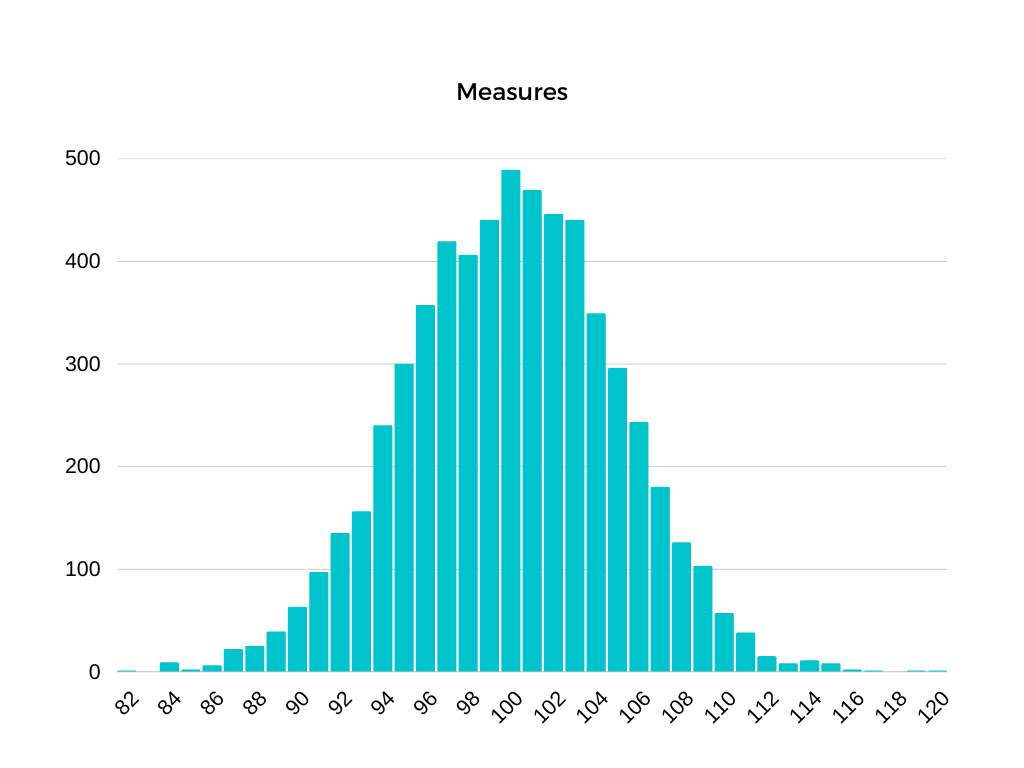
\includegraphics{pics/Measures.png}

It is clear how they describe the behaviour of a normal distribution.

\hypertarget{and-then-the-histogram-of-the-predicted-values-for-the-y-component}{%
\subparagraph{And then the histogram of the predicted values (for the y
component):}\label{and-then-the-histogram-of-the-predicted-values-for-the-y-component}}

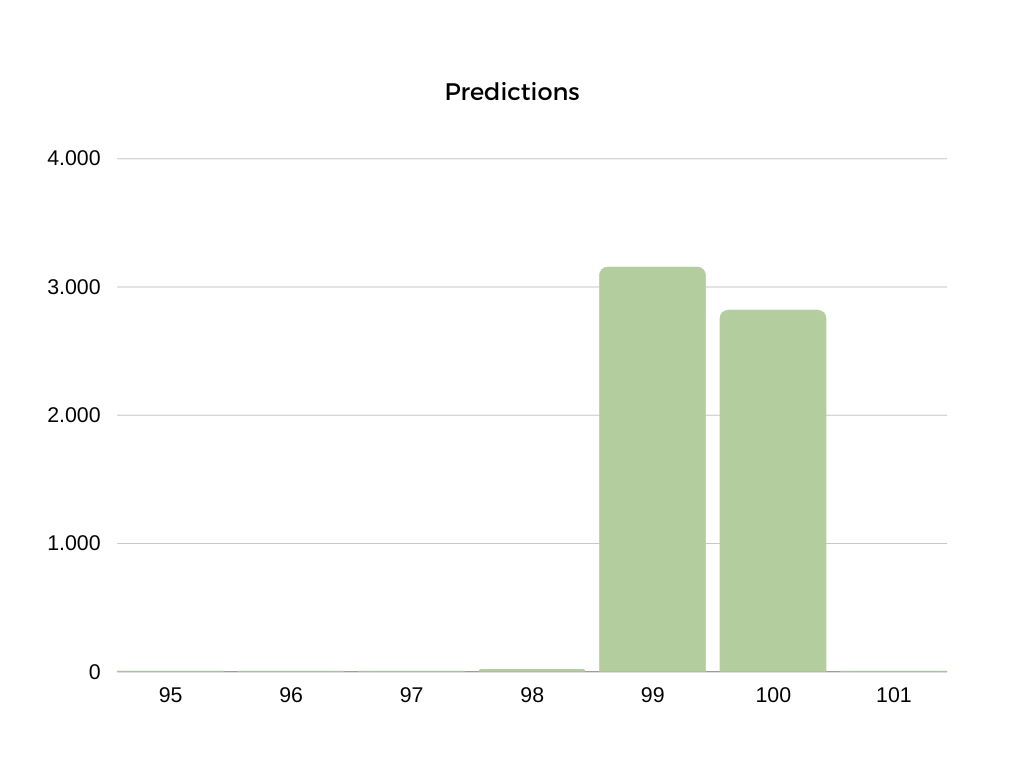
\includegraphics{pics/Predictions.png}

The filter was able to reduce the noise coming from the encoders!

\hypertarget{case-study}{%
\subsection{Case study}\label{case-study}}
